\section{Evaluation}\label{eval}

%In this section, we perform testbed experiments to evaluate \sysname. 
%We highlight our findings as follows.

% \begin{itemize}[leftmargin=*]
% %
%     \item Compared to a wide spectrum of baselines, \sysname provides $3.3\times$ higher accuracy to various applications. Compared to sketch-only baselines, \sysname achieves at least $3.3\times$ higher accuracy when measuring small flows. Compared to INT-only baselines, \sysname reduces at least $3.3\times$ overheads in network bandwidth and control plane resources. Compared to hybrid baselines, \sysname improves accuracy by 3.3$\times$. 
% %
%     \item \sysname offers the near-optimal measurement point selection that improves the flow coverage by $3.7\times \sim 3.8\times$ and reduces the distance between switches and control plane nodes by $3.7\times \sim 3.8\times$ when compared to strawman approaches such as heuristics. It also maintains timeliness that quickly yields decisions within a few milliseconds. 
% %
%     \item \sysname eliminates network congestion via its loss-free measurement data collection. Its dynamic path selection prevents high link utilization in all cases, while existing solutions fail to avoid data loss when dynamics occur. 
% %
% \end{itemize}

\subsection{Experimental Setup}\label{setup}

\para{Implementation}. Our implementation comprises optimization algorithms and a controller. For the optimization algorithms, we implement the Lagrangian relaxation algorithms for measurement point selection (\S\ref{selection}) in C++ using the Gurobi API \cite{gurobi}. The RL algorithm for congestion-free data collection (\S\ref{collection}) is implemented using PyTorch with the CPO library \cite{pytorch}. Next, we implement a controller in Python that translates optimization outputs (i.e., \(x_p\), \(y_p\), \(z_{p,c}\) variables) into switch configurations. Specifically, it configures: (1) sketch deployment and INT activation on selected switches via data plane program deployment \cite{chen2020speed,gao2020lyra}, and (2) data routing rules inside match-action tables to direct measurement data to target paths. The controller uses the Tofino SDE \cite{tofino2} to load configurations on switches.

\para{Testbed and simulator}. We construct a real testbed comprising six \(64 \times 400\)\,Gbps Tofino2 programmable switches \cite{tofino2}. These switches are interconnected within a two-level fat-tree topology via 100-Gbps links. Also, at the network edge, we establish a cluster of high-performance servers, each offering 36-core Intel Xeon Gold 6240C 2.60\,GHz CPU and 128-GB RAM, as the control plane. For traffic generation, we connect eight servers that runs PktGen-DPDK \cite{pktgen} at line rate to the network. Next, due to limited testbed scale, we implement a C++ simulator to simulate large-scale topologies that models: (1) switch pipelines with resource constraints \cite{jose2015compiling}, (2) link bandwidths and latency, and (3) switch and control-plane performance statistics based on real-world measurements. The simulator accepts real traffic traces such as CAIDA \cite{caida} and topology files as input.

\para{Topologies and workloads}. We simulate two typical classes of topologies \cite{anup2022hetero,chen2024eagle}. (1) Wide-area networks (WANs). We select five WANs, AboveNet (20 switches), Internet2 (42 switches), ForthNet (62 switches), Bestel (83 switches), and Interroute (109 switches), from the Internet topology zoo \cite{knight2011internet}. We denote these topologies with T1-T5. We set the transmission latency of each link to be randomly distributed between 10\,ms to 50\,ms while setting all switches to be programmable. (2) Data center networks (DCNs). For DCNs, we consider the fat-tree networks and vary the pod number: C1-C5 that use 16, 20, 24, 32, and 48 pods, respectively, e.g., C5 has 2880 switches and 55296 links. We set the link latency to be randomly varied between 1\,$\mu$s to 10\,$\mu$s. We randomly pick 30\% of switches to be programmable based on recent statistics \cite{telecom}. For each programmable switch, we set its configurations based on real switches \cite{jose2015compiling}.

For control plane nodes, we leverage two distinct strategies for WANs and DCNs, respectively. For WANs, we employ the technique that optimizes the placement of control plane nodes in WANs \cite{heller2012controller}. For DCNs, we allocate a distinct control plane node to each pod of fat-tree networks. 

We choose corresponding workloads that match WANs and DCNs. For WANs, we choose a CAIDA trace \cite{caida} that lasts for one minute and comprises around 26\,M packets. For DCNs, we use the complete IMC DCN traffic trace \cite{benson2010network}. Each flow's OD pair is randomly selected among edge switches. 

\begin{figure}[t]
    \centering
    \begin{subfigure}{0.49\linewidth}
    \centering
    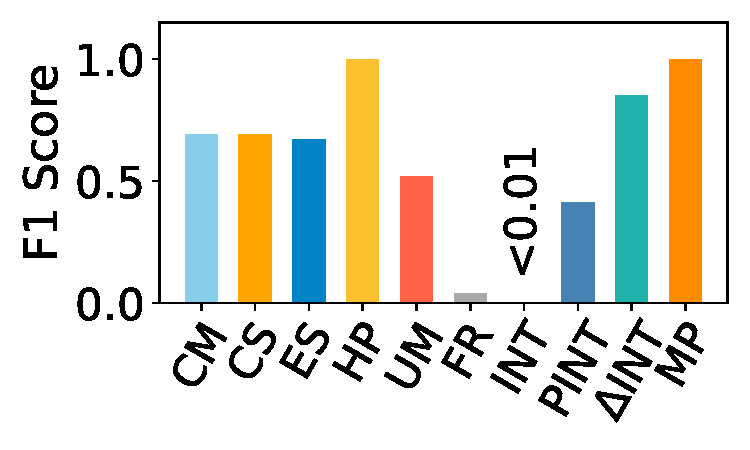
\includegraphics[width=\linewidth]{pics/hhF1-caida.pdf}
    \vspace{-20pt}
    \caption{HH (CAIDA).}
    \end{subfigure}
    \begin{subfigure}{0.49\linewidth}
    \centering
    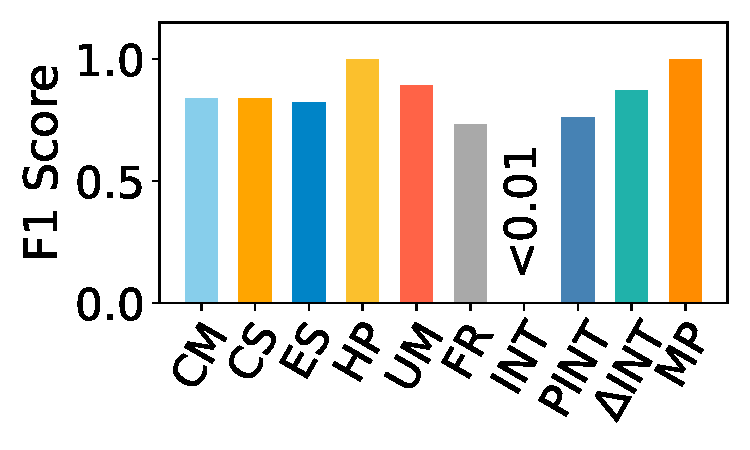
\includegraphics[width=\linewidth]{pics/hhF1-imc.pdf}
    \vspace{-20pt}
    \caption{HH (IMC).}
    \end{subfigure}
    
    \begin{subfigure}{0.49\linewidth}
    \centering
    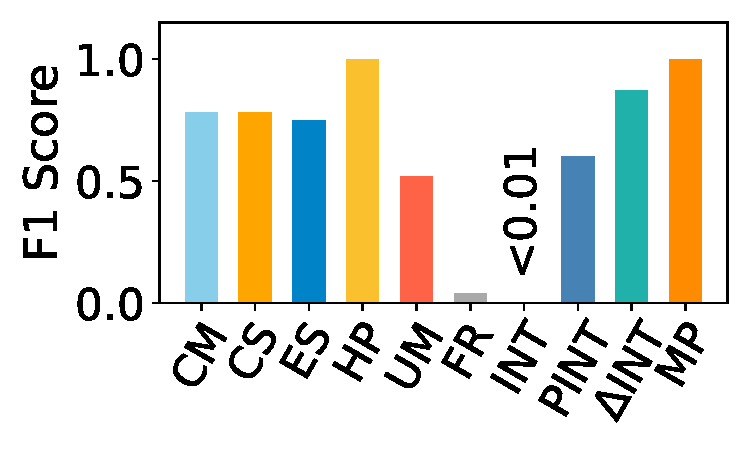
\includegraphics[width=\linewidth]{pics/ssF1-caida.pdf}
    \vspace{-20pt}
    \caption{SS (CAIDA).}
    \end{subfigure}
    \begin{subfigure}{0.49\linewidth}
    \centering
    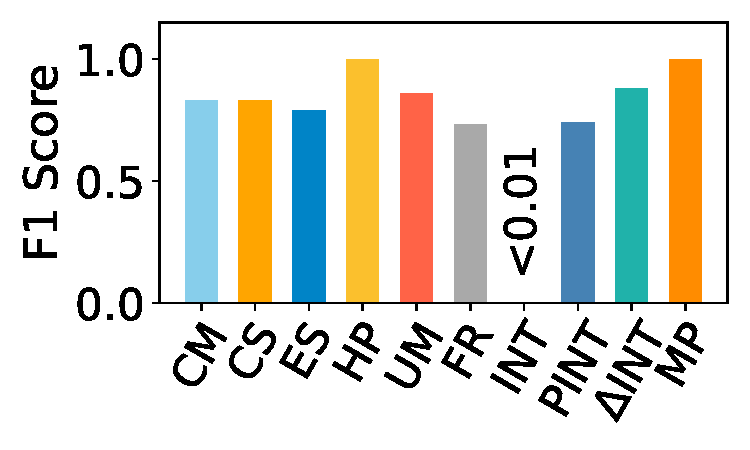
\includegraphics[width=\linewidth]{pics/ssF1-imc.pdf}
    \vspace{-20pt}
    \caption{SS (IMC).}
    \end{subfigure}
    
    \begin{subfigure}{0.49\linewidth}
    \centering
    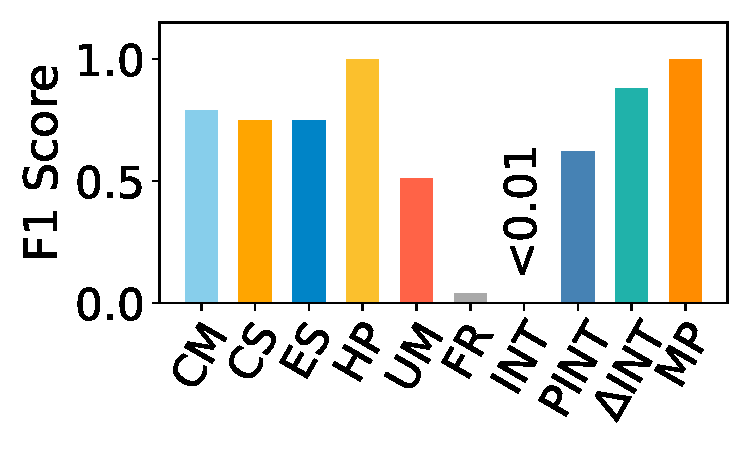
\includegraphics[width=\linewidth]{pics/dfF1-caida.pdf}
    \vspace{-20pt}
    \caption{DF (CAIDA).}
    \end{subfigure}
    \begin{subfigure}{0.49\linewidth}
    \centering
    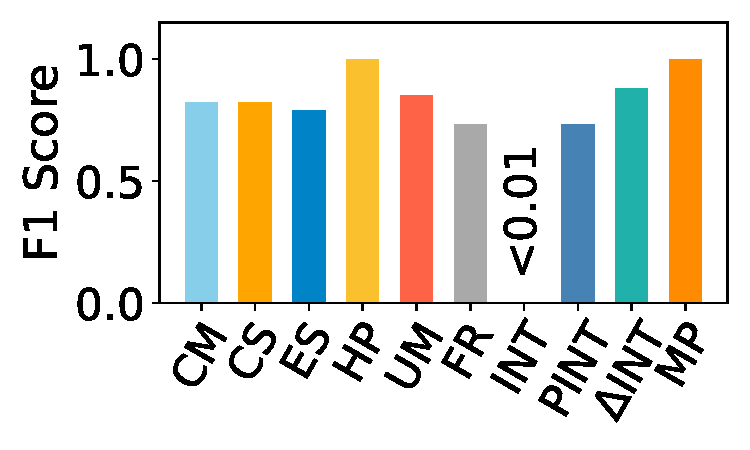
\includegraphics[width=\linewidth]{pics/dfF1-imc.pdf}
    \vspace{-20pt}
    \caption{DF (IMC).}
    \end{subfigure}

    \begin{subfigure}{0.49\linewidth}
    \centering
    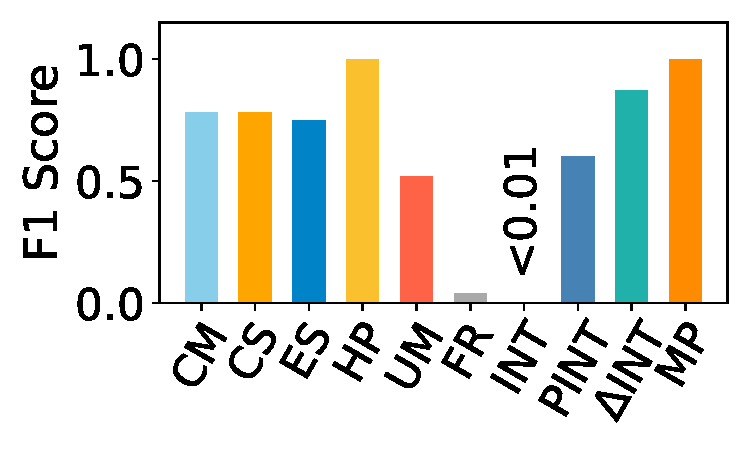
\includegraphics[width=\linewidth]{pics/ssF1-caida.pdf}
    \vspace{-20pt}
    \caption{SS (CAIDA).}
    \end{subfigure}
    \begin{subfigure}{0.49\linewidth}
    \centering
    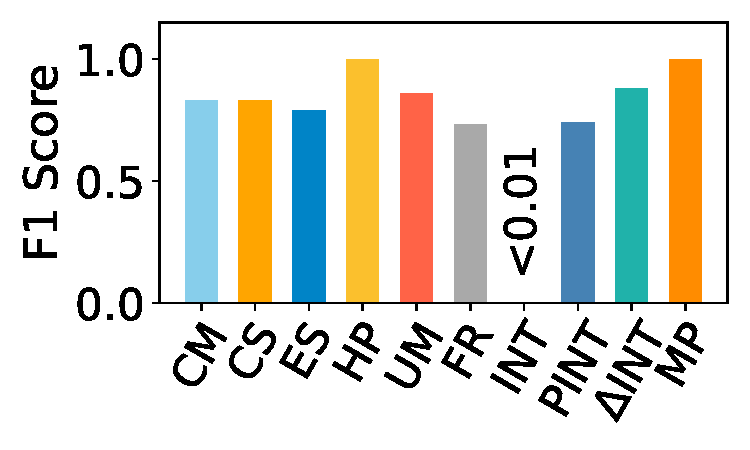
\includegraphics[width=\linewidth]{pics/ssF1-imc.pdf}
    \vspace{-20pt}
    \caption{SS (IMC).}
    \end{subfigure}
    
    \begin{subfigure}{0.49\linewidth}
    \centering
    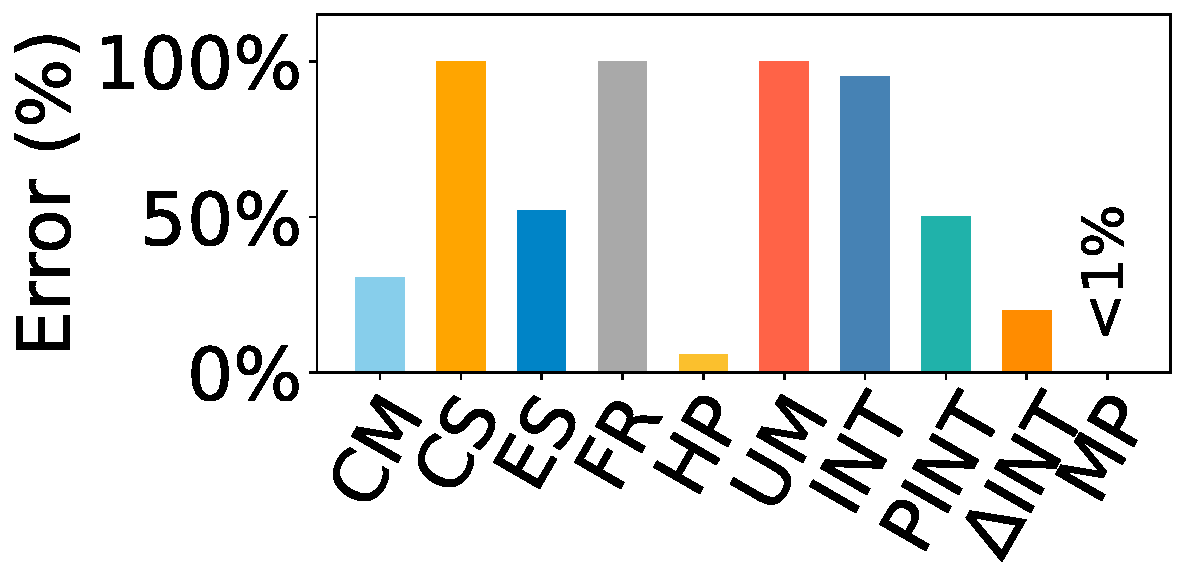
\includegraphics[width=\linewidth]{pics/pc-caida.pdf}
    \vspace{-20pt}
    \caption{PC (CAIDA).}
    \end{subfigure}
    \begin{subfigure}{0.49\linewidth}
    \centering
    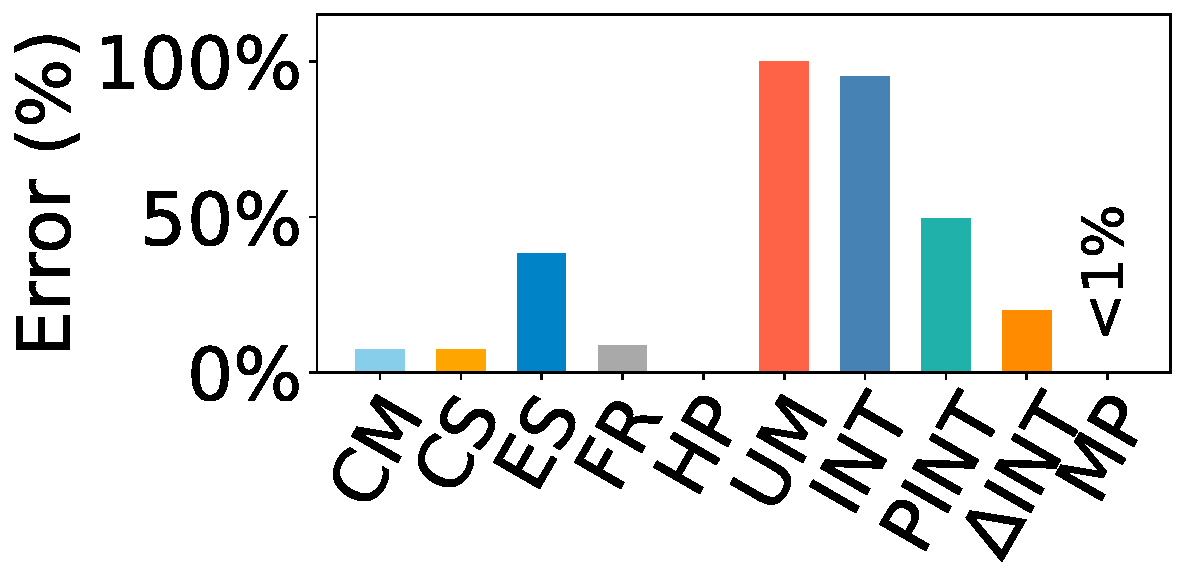
\includegraphics[width=\linewidth]{pics/pc-imc.pdf}
    \vspace{-20pt}
    \caption{PC (IMC).}
    \end{subfigure}
    \caption{Accuracy for volumetric applications.}
    \vspace{-2pt}
    \label{fig:volumetric-acc}
\end{figure}

\begin{figure}[t]
    \centering
    \begin{subfigure}{0.49\linewidth}
    \centering
    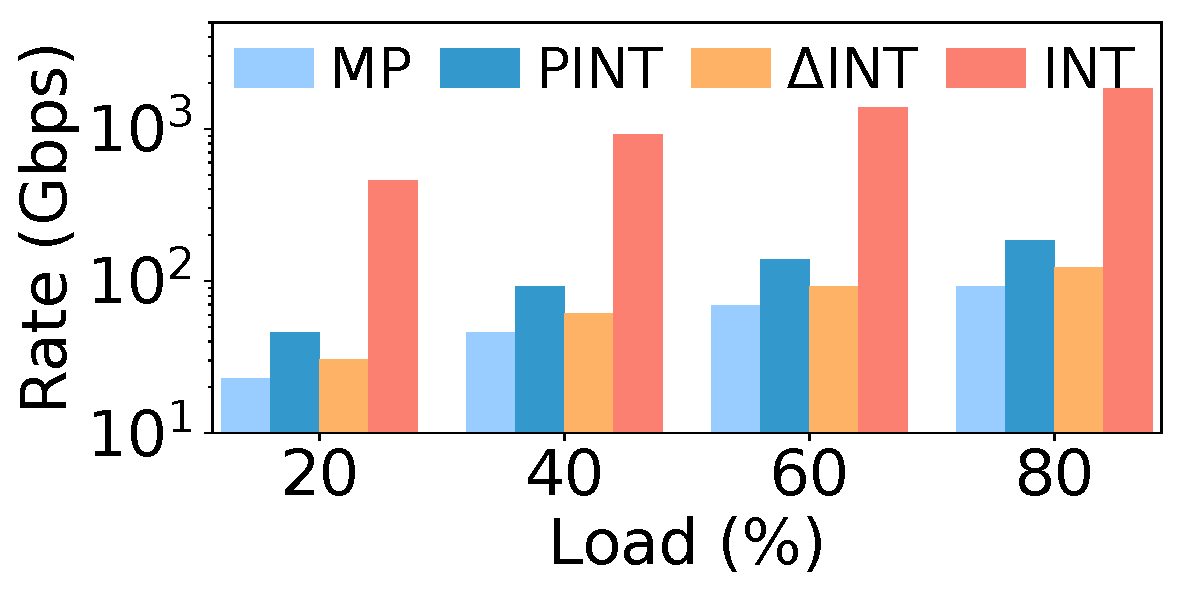
\includegraphics[width=\linewidth]{pics/pc-rate.pdf}
    \vspace{-20pt}
    \caption{Sending rate.}
    \end{subfigure}
    \begin{subfigure}{0.49\linewidth}
    \centering
    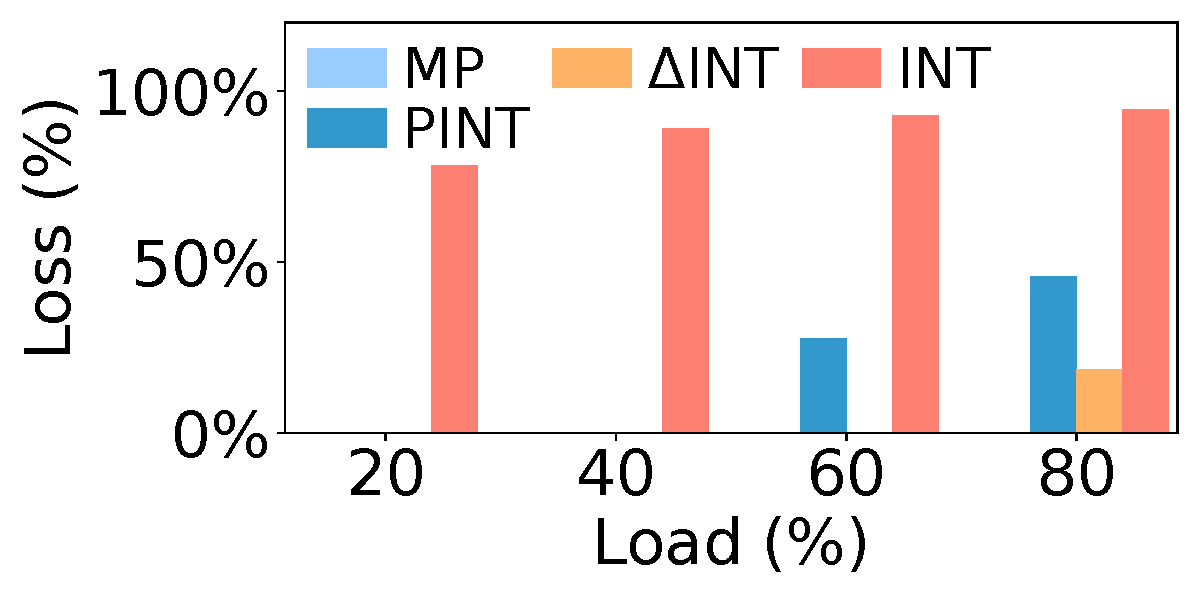
\includegraphics[width=\linewidth]{pics/pc-loss.pdf}
    \vspace{-20pt}
    \caption{Data loss.}
    \end{subfigure}
    \caption{Overheads for volumetric applications.}
    \vspace{-2pt}
    \label{fig:volumetric-loss}
\end{figure}

\begin{figure}[t]
    \centering
    \begin{subfigure}{0.7\linewidth}
    \centering
    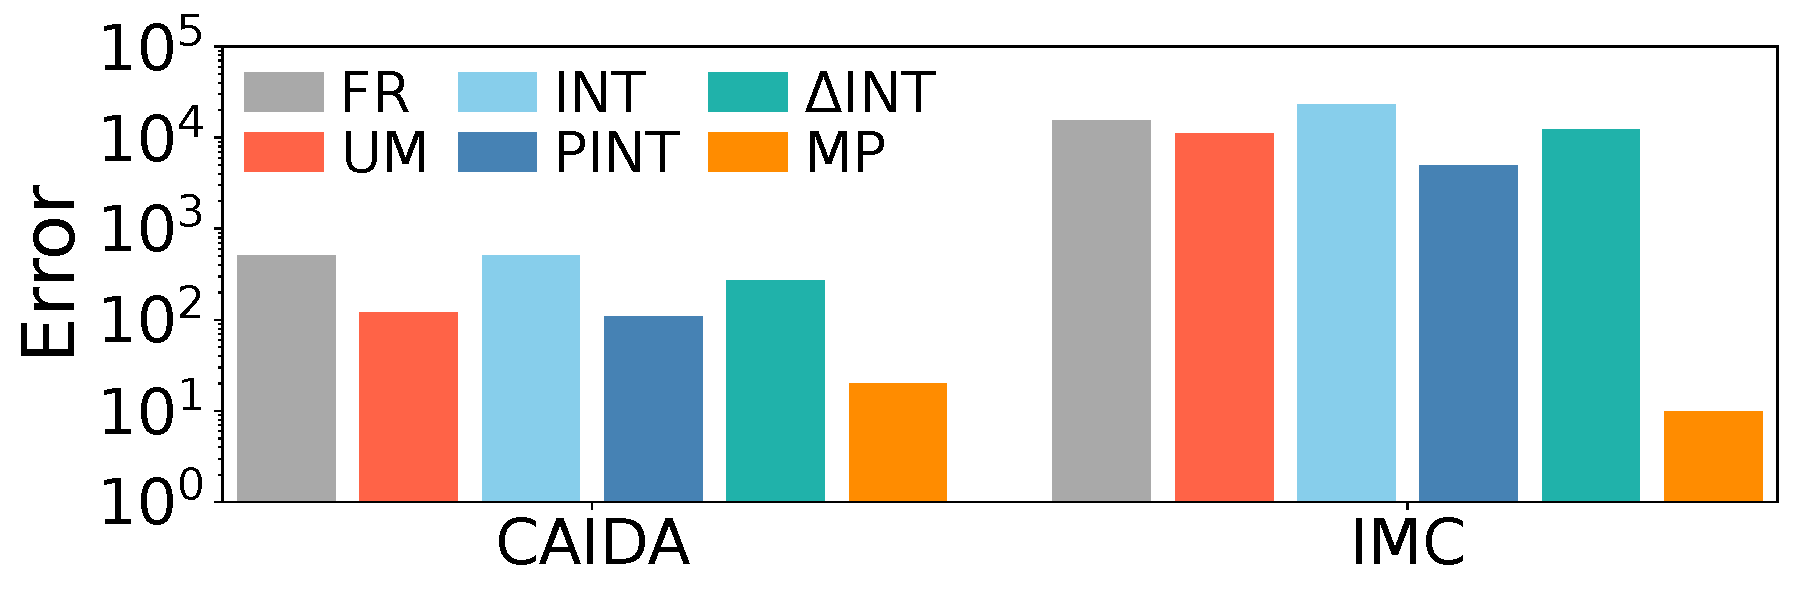
\includegraphics[width=\linewidth]{pics/ee.pdf}
    \vspace{-20pt}
    \caption{EE.}
    \end{subfigure}
    \begin{subfigure}{0.28\linewidth}
    \centering
    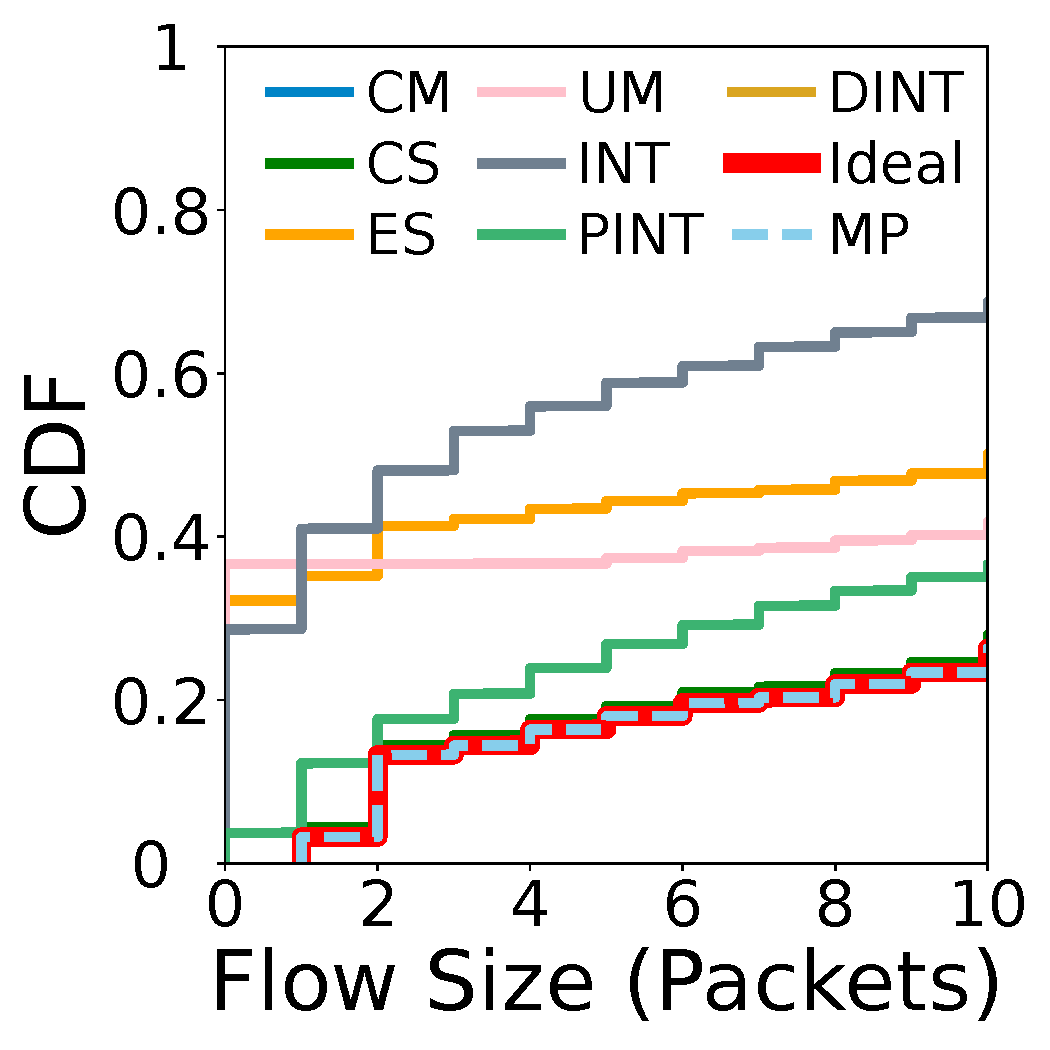
\includegraphics[width=\linewidth]{pics/cdf-imc.pdf}
    \vspace{-18pt}
    \caption{FD.}
    \end{subfigure}
    \caption{Accuracy for aggregated applications.}
    \vspace{-2pt}
    \label{fig:aggregated-acc}
\end{figure}

%We realize them with CM, CS, ES, FR, HP, and UM, respectively. We realize EE with FR, MARC, and UM, respectively.

\para{Baselines}. We compare \sysname with five types of techniques. 

\begin{itemize}[leftmargin=*]
%
    \item[1] \textbf{Sketches only}. We implement six state-of-the-art sketches, including the count-min sketch (CM) \cite{cormode2005improved}, the count sketch (CS) \cite{charikar2004finding}, the elastic sketch (ES) \cite{yang2018elastic}, FlowRadar (FR) \cite{li2016flowradar}, HashPipe (HP) \cite{sivaraman2017heavy}, and UnivMon (UM) \cite{liu2016one}. We also refer to the theoretical bounds in their original papers to configure their parameters to maximize accuracy. % sketches = c++
%
    \item[2] \textbf{INT only}. We consider three classic INT techniques, including the original INT \cite{int}, PINT \cite{ben2020pint}, and DeltaINT \cite{sheng2021deltaint}. We implement them based on their open-source implementations. % int, pint (sampling rate = 0.X), deltaint (see paper)
%
    \item[3] \textbf{Hybrid sketch+INT}. Recall from \S\ref{hybrid}, we implement the open-source SketchINT \cite{yang2023sketchint} and LightGuardian \cite{zhao2021lightguardian}. 
%
    \item[4] \textbf{Measurement point selection algorithms}. We choose three algorithms for selecting measurement points, i.e., MTP \cite{chen2021mtp} that aims to minimize the number of occupied measurement points to place sketches and INT, SPEED \cite{chen2020speed} that optimizes both resources and performance, and a Greedy-based heuristic that prioritizes the switches with more resources. 
%
    \item[5] \textbf{Data collection path selection algorithms}. We use three algorithms for selecting the paths of transferring measurement data, i.e., Escala \cite{liu2022escala} that selects the paths with lower latency, a randomized algorithm that randomly chooses its paths, and INT-path \cite{pan2019int} that adopts a depth-first search (DFS) heuristic to cover as many measurement points as possible.
%
\end{itemize}

For a fair comparison, we set the top three types of techniques to select the same measurement points and paths chosen by the algorithms of \sysname. We fix the amount of switch memory allocated to each sketch or INT to 10\,MB, which is close to the maximum capacity of a switch \cite{gupta2018sonata}. 
Moreover, to quantify the solution quality of the last two types of techniques, we also use Gurobi \cite{gurobi} to find the optimal decisions (i.e., OPT). 

\para{Applications}. We consider three types of network management applications based on their differences on queries.

%(1) volumetric applications, i.e., heavy hitter detection (HH) \cite{huang2017sketchvisor}, superspreader detection (SS) \cite{tang2019mv}, DDoS flow detection (DF) \cite{liu2021jaqen}, and per-flow packet counting (PC) (2) aggregated applications, i.e., entropy estimation (EE) \cite{liu2016one}, and (3) troubleshooting applications, i.e., path monitoring (PM) \cite{ben2020pint,sheng2021deltaint}. According to the literature, we set the thresholds of HH to 10K packets and set the threshold of SS to 0.5\% of the total number of IP addresses. Also, for EE, we compute the entropy of measured flow distributions based on \cite{liu2016one}. These applications run on the control plane, which installs an instance on each server to collectively handle input data. 

% \noindent With the above terms, we classify network management applications into three classes based on their differences on queries.

\begin{itemize}[leftmargin=*]
%
    \item Volumetric applications include heavy hitter detection (HH) \cite{huang2017sketchvisor}, superspreader detection (SS) \cite{tang2019mv}, DDoS flow detection (DF) \cite{liu2021jaqen}, and per-flow packet counting (PC) \cite{huang2017sketchvisor} and query the size of each flow. 
%
    \item Aggregated applications include entropy estimation (EE) \cite{liu2016one} and flow size distribution (FD) \cite{chen2021mtp} that aggregate statistics to summarize all flows. %For FD, we set the flow identifier to two-tuple and five-tuple, respectively.
%
    \item Troubleshooting applications, e.g., latency monitoring (LM) and congestion control (CC) \cite{ben2020pint,sheng2021deltaint}, query per-flow metadata (i.e., timestamps and queue lengths).
%
\end{itemize}

\noindent According to their differences, we use different baselines: (1) Volumetric applications focus on large flows while aggregated applications consider all flows. As such, we compare \sysname with sketches-only, INT-only, and hybrid baselines. (2) Troubleshooting applications rely on INT data, such that we only compare \sysname with INT-only and hybrid baselines. For the solutions that combine both sketches and INT, we use the sketch that yields the best results for a fair comparison. 

\subsection{Benefits of \sysname}

\para{\sysname brings accuracy and efficiency benefits to diverse applications}. 
In our testbed, we use \sysname and baselines to measure traffic, respectively. We continuously replay CAIDA traces \cite{caida} to our testbed and set the OD pair of each flow to random edge switches. The control plane runs the applications in \S\ref{setup} to identify the flows of their interest based on collected data. We compute the accuracy by comparing measured data with the ground truth obtained by analyzing input traces. 

% figure a-e: x = f1 + recall + precision, y = ratio (%), lines = monplan, sketch (cm,cs,...), int, pint, deltaint
% trace: caida 2018
% figure a = HH, figure b = SS, figure c = DF, figure d = EE, figure e = PM
% each figure occupies a complete line

\noindent \emph{(1) Evaluation with volumetric applications}

According to the literature, we set the thresholds of HH to 10K packets, set the threshold of SS to 0.5\% of the total number of IP addresses, and set the threshold of DF to 0.5\% of the total number of five-tuples. PC considers per-flow packet counts. We adopt the F1 score, 2\emph{tp}/(2\emph{tp}+\emph{fp}+\emph{fn}), where \emph{tp}, \emph{fp}, and \emph{fn} denote the number of true positives, false positives, and false negatives. 

%the precision, \emph{tp}/(\emph{tp}+\emph{fp}), the recall, \emph{tp}/(\emph{tp}+\emph{fn}), and 

For HH, SS, DF, in Figure~\ref{fig:volumetric-acc}, \sysname achieves $3.3\times$ higher accuracy. This advantage originates from co-designing sketches and INT: sketches enable accurate measurement for large flows while INT mitigate the errors of measuring small flows, while using only sketches or INT alone drops accuracy: small flows in sketches suffer from hash collisions with large flows, while direct INT brings congestion and data loss. 

%Next, we fix the threshold of distinguishing large and small flows to 10K packets and quantify the errors of measuring small flows. 
For PC, in Figure~\ref{fig:volumetric-acc}, \sysname achieves near-optimal accuracy because it employs fully accurate INT for small flows, which outperforms existing sketches by $3.3\times$.  

% figure a: x = sketches, y = f1, lines = monplan, sketches-only
% figure b: x = sketches, y = recall, lines = monplan, sketches-only
% trace: small flows in caida 2019=8
% each figure occupies a half line (two figures per line)

Figure~\ref{fig:volumetric-loss} presents the overheads of \sysname when transfering data to the control plane. Compared with INT, \sysname reduces the rate of transferring data by two orders of magnitude when we manually increase traffic rate from 20\% to 80\% of switch capability. Such a benefit comes from our design that only small flows trigger INT, thus limiting overheads and avoids data loss. 

% figure a (see excalibur paper): x = 100Gbps - 1Tbps, y = INT rate, lines = monplan, int, pint, deltaint 
% figure b: x = 100Gbps - 1Tbps, y = loss rate, lines = monplan, int, pint, deltaint 
% note: link 100 Gbps, estimate measurement data sending rate and compute loss rate
% each figure occupies a half line (two figures per line)

\noindent \emph{(2) Evaluation with aggregated applications}

For EE, we only consider FR and UM since only those two sketch-only baselines support EE. Figure~\ref{fig:aggregated-acc} shows that \sysname reduces its estimation errors and produces an entropy near the true one. Again, this improvement comes from the accuracy of measuring small flows via INT in \sysname. 

For FD, we change the flow identifier to two-tuple and five-tuple, respectively. In Figure~\ref{fig:aggregated-acc}, \sysname produces near-optimal distributions because it well preserves the high accuracy of per-flow packet counts. In contrast, other baselines suffer from non-trivial accuracy loss due to the miss of small flows or data loss incurred by congestions during measurement data transmission. 

\noindent \emph{(3) Evaluation with troubleshooting applications}

For LM, we collect the medium and tail latency for \emph{(switch, flow)} pairs. We replay the Web search \cite{alizadeh2010data} and Hadoop workloads \cite{roy2015inside} in our testbed. Moreover, we follow \cite{ben2020pint} to use KLL \cite{karnin2016optimal}, a quantitive algorithm, to analyze latencies in the control plane. We consider the average relative error (ARE) of the 50th and 99th percentile latencies. Figure 10 shows that \sysname optimizes the ARE for the 50th percentile latencies of PINT by up to 33\%, and decreases the ARE for the 99th percentile latencies of DeltaINT by up to 33\%. This is because \sysname carefully selects network paths to transfer measurement data, which avoids data loss and preserves application-level accuracy.

For CC, we exploit HPCC \cite{li2019hpcc} for congestion control that adjusts the servers' sending rates with respect to collected link utilization. We reuse the same workloads as the LM experiment. The metric we use to evaluate congestion control is \emph{slowdown}, which equals the ratio between the completion time of a flow when all other flows exist and when only the flow itself exists. A smaller slowdown corresponds to better congestion control. We consider the 95th percentile slowdown for each flow size. Figure 10 demonstrates that \sysname achieves more accurate congestion control. In contrast, due to the loss of collected link utilization, PINT and DeltaINT fail to adjust sending rates. 

\subsection{Microbenchmarks}

%Next, to quantify the effectiveness of \sysname, we stress-test \sysname's algorithms with large-scale simulations. 

\para{\sysname achieves near-optimal measurement point selection}. We invoke \sysname and the comparison solutions to select measurement points in WANs and DCNs, respectively. Figure~6 presents the flow coverage of decisions made by each technique. It indicates that \sysname covers most flows even with unknown routing information, while other techniques fail to provide high coverage. Our algorithms also optimize the distances between switches and control plane nodes, yielding near-optimal results. 

We also measure the execution time of \sysname. Figure~6 indicates that through Lagrangian relaxation, \sysname reduces the time by orders of magnitude when compared with OPT. 

% set the number of flows to the trace used in WANs or DCNs
% set flows with random od pairs
% figure a: x = topologies, y = coverage, lines = monplan, mtp, speed, greedy, OPT (Gurobi)
% figure b: x = topologies, y = avg. distance (# hops), lines = monplan, mtp, speed, greedy, OPT (Gurobi)
% figure c: x = topologies, y = time, lines = monplan, mtp, speed, greedy, OPT (Gurobi)

\para{\sysname achieves near-optimal data collection path selection}. We invoke \sysname and the comparison solutions to select network paths for transferring measurement data, respectively. Figure~7 computes the number of congested links incurred by the decisions made by each technique. \sysname prevents link congestions in its collection, while other techniques bring non-trivial congestions, leading to high data loss rates of 23$\sim$33\%. Also, its RL algorithm maintains timeliness, which selects paths within a few milliseconds. Hence, it is acceptable for handling runtime dynamics with loss-free measurement data collection. 

%We also measure the execution time of \sysname. Figure~6 indicates that through Lagrangian relaxation, \sysname reduces the time by orders of magnitude when compared with OPT. 

% set the number of flows to the trace used in WANs or DCNs
% set flows with random od pairs
% figure a: x = topologies, y = # of congested links, lines = monplan, escala, int-path, OPT (Gurobi)
% figure b: x = topologies, y = loss rate, lines = monplan, escala, int-path, OPT (Gurobi)
% figure c: x = topologies, y = time, lines = monplan, escala, int-path, OPT (Gurobi)

